\documentclass[14pt,aspectratio=169]{beamer}
\usepackage[utf8]{inputenc}
\usepackage{wasysym}
\usepackage{svg}
\usepackage{amsmath}
\usepackage{amssymb}
\usepackage{fourier}
\usepackage{physics}

\usepackage{minted}
\usemintedstyle{tango}

\usefonttheme{professionalfonts}

\mode<presentation>

\usetheme{Antibes}
\usecolortheme{seagull}

\setbeamertemplate{navigation symbols}{}
\setbeamertemplate{headline}{} % hide navbar
\setbeamertemplate{footline}[frame number]

\title{Scientific Machine Learning \\ Final Project}
\author{Lovnesh Bhardwaj, Laurynas Varnas}
\date{}

\begin{document}

\begin{frame}
	\titlepage
\end{frame}

\begin{frame}[plain]
	\centering
	\usebeamercolor[fg]{title}\usebeamerfont{title}
	Finite Element Method
\end{frame}

\begin{frame}{Problem definition}
	Monodomain equation
	\begin{align*}
		\pdv{u}{t} - \divergence \Sigma \grad u + f(u) & = 0   & \text{in } \Omega \times I,          \\
		\mathbf{n} \cdot \grad u                       & = 0   & \text{on } \partial \Omega \times I, \\
		u                                              & = u_0 & \text{in } \Omega \times \{0\},
	\end{align*}
\end{frame}

\begin{frame}{IMEX}
	With $U^n(x) \approx u(x, t_n)$
	\begin{align*}
		\frac{U^{n+1} - U^n}{\Delta t}                        & = \divergence \Sigma \grad U^{n+1} - f(U^n) \\
		\\
		U^{n+1} - \Delta t\, \divergence \Sigma \grad U^{n+1} & = U^n - \Delta t\, f(U^n)
	\end{align*}
\end{frame}

\begin{frame}{Algebraic formulation of the FEM discretization}

	\begin{align*}
		(\mathbf M + \Delta t\, \mathbf K)\, \mathbf u^{n+1} = \mathbf M\, \mathbf u^n - \Delta t\, \mathbf f(U^n),
	\end{align*}

	where:

	\begin{align*}
		\mathbf M_{ij}   & = \int_\Omega \phi_i(x) \phi_j(x)\,\diffd x \quad                             & \text{(mass matrix)},           \\
		\mathbf K_{ij}   & = \int_\Omega \Sigma(x) \grad \phi_i(x) \cdot \grad \phi_j(x)\,\diffd x \quad & \text{(stiffness matrix)},      \\
		\mathbf f_i(U^n) & = \int_\Omega f(U^n(x)) \phi_i(x)\,\diffd x \quad                             & \text{(nonlinear load vector)}.
	\end{align*}
\end{frame}

\begin{frame}[plain]
	\centering
	\usebeamercolor[fg]{title}\usebeamerfont{title}
	FEM Results
\end{frame}

\begin{frame}
	\centering
	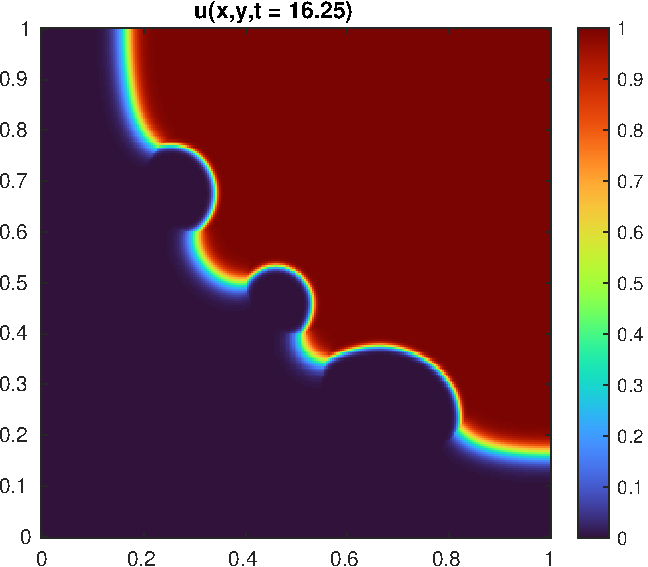
\includegraphics[height=\textheight]{figs/S01.pdf}
\end{frame}

\begin{frame}
	\centering
	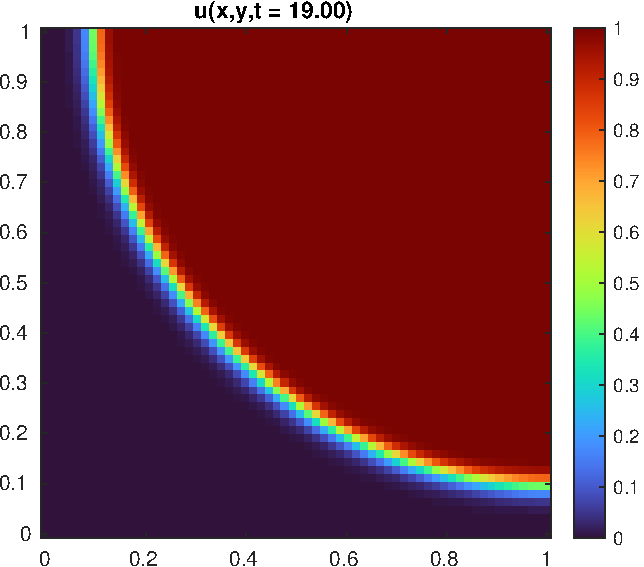
\includegraphics[height=\textheight]{figs/S1.pdf}
\end{frame}

\begin{frame}
	\centering
	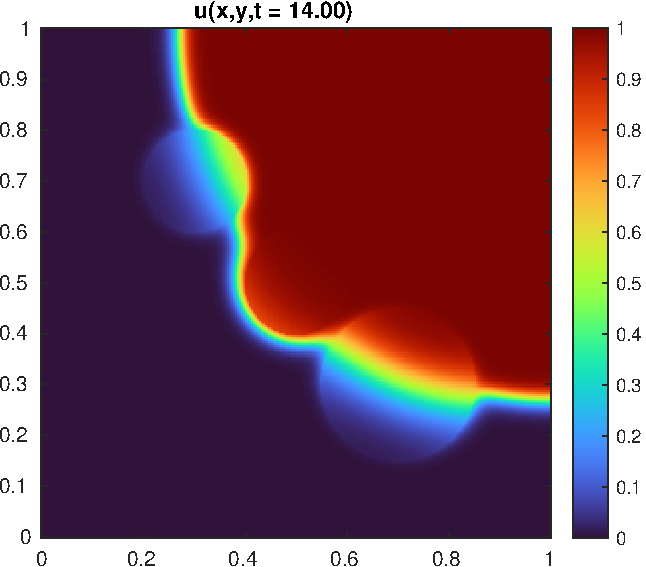
\includegraphics[height=\textheight]{figs/S10.pdf}
\end{frame}

\begin{frame}{$\Sigma_d = 10$}
	\begin{table}[H]
		\centering
		\begin{tabular}{l|r|ccc}
			$\Delta t$ & $n_e$ & Activation time & M-matrix?     & $u \in [0, 1]$ \\
			\hline
			0.1        & 64    & 28.60           & \textbf{true} & false          \\
			0.1        & 128   & 29.10           & \textbf{true} & false          \\
			0.1        & 256   & 29.20           & \textbf{true} & false          \\
			0.05       & 64    & 26.60           & false         & false          \\
			0.05       & 128   & 27.15           & \textbf{true} & \textbf{true}  \\
			0.05       & 256   & 27.20           & \textbf{true} & \textbf{true}  \\
			0.025      & 64    & 25.60           & false         & false          \\
			0.025      & 128   & 26.10           & \textbf{true} & \textbf{true}  \\
			0.025      & 256   & 26.175          & \textbf{true} & \textbf{true}  \\
		\end{tabular}
	\end{table}
\end{frame}

\begin{frame}{$\Sigma_d = 1$}
	\begin{table}[H]
		\centering
		\begin{tabular}{l|r|ccc}
			$\Delta t$ & $n_e$ & Activation time & M-matrix?     & $u \in [0, 1]$ \\
			\hline
			0.1        & 64    & 30.20           & \textbf{true} & false          \\
			0.1        & 128   & 30.90           & \textbf{true} & false          \\
			0.1        & 256   & 31.00           & \textbf{true} & false          \\
			0.05       & 64    & 28.10           & false         & false          \\
			0.05       & 128   & 28.80           & \textbf{true} & \textbf{true}  \\
			0.05       & 256   & 28.90           & \textbf{true} & \textbf{true}  \\
			0.025      & 64    & 27.025          & false         & false          \\
			0.025      & 128   & 27.70           & \textbf{true} & \textbf{true}  \\
			0.025      & 256   & 27.775          & \textbf{true} & \textbf{true}  \\
		\end{tabular}
	\end{table}
\end{frame}

\begin{frame}{$\Sigma_d = 0.1$}
	\begin{table}[H]
		\centering
		\begin{tabular}{l|r|ccc}
			$\Delta t$ & $n_e$ & Activation time & M-matrix?     & $u \in [0, 1]$ \\
			\hline
			0.1        & 64    & 31.70           & false         & false          \\
			0.1        & 128   & 32.50           & false         & false          \\
			0.1        & 256   & 32.60           & \textbf{true} & false          \\
			0.05       & 64    & 29.55           & false         & false          \\
			0.05       & 128   & 30.25           & false         & false          \\
			0.05       & 256   & 30.40           & false         & \textbf{true}  \\
			0.025      & 64    & 28.40           & false         & false          \\
			0.025      & 128   & 29.075          & false         & false          \\
			0.025      & 256   & 29.225          & false         & \textbf{true}  \\
		\end{tabular}
	\end{table}
\end{frame}

\end{document}
